%%%%%%%%%%%%%%%%%%%%%%%%%%%%%%%%%%%%%%%%%%%%%%%%%%%%%%%%%%%%%%%%%%%%%%%%%%%%%
%% Descr:       Vorlage für Berichte der DHBW-Karlsruhe, Ein Kapitel
%% Author:      Prof. Dr. Jürgen Vollmer, vollmer@dhbw-karlsruhe.de
%% $Id: kapitel2.tex,v 1.5 2017/10/06 14:02:51 vollmer Exp $
%%  -*- coding: utf-8 -*-
%%%%%%%%%%%%%%%%%%%%%%%%%%%%%%%%%%%%%%%%%%%%%%%%%%%%%%%%%%%%%%%%%%%%%%%%%%%%%%%

%\section{OpenGL}
%\label{chap:OpenGL}
%\subsection{Projektionen}
%\subsection{Shader}

\section{Softwarearchitektur}
\label{chap:Softwarearchitektur}
Komponenten in Form von Klassen, Objekten oder Bibliotheken und deren Verbindungen zwischen einzelnen Komponenten beschreibt die Architektur 
eines Softwaresystems. Vielmehr geht es bei der Software-Architektur darum, Anforderungen und deren Zusammenhänge untereinander von dem zu 
konstruierenden System zu beschreiben und nicht einen detaillierten Entwurf vorzulegen. Jedoch hat die Architektur einen enormen Einfluss 
auf die qualitativen und nicht-funktionalen Eigenschaften des daraus resultierenden Systems. 
\\ 
\linebreak
Die Terminologie nach dem \textit{IEEE-Standard 1471-2000} zur Software Architekturbeschreibung, deren Aufgaben und Zweck \cite{swarchitekturieee.2005} 
sind wie folgt definiert: 
\begin{quote}
    Die grundlegende Organisation eines Systems, dargestellt durch dessen Komponenten, deren Beziehungen zueinander und zur Umgebung sowie den 
    Prinzipien, die den Entwurf und die Evolution des Systems bestimmen. \cite{architektursw.2006f}
\end{quote}
Softwarearchitektur bietet viele Möglichkeiten ein System zu entwerfen und Anforderungen und Eigenschaften umzusetzen, daher gibt es auch 
hier viele Ansätze, Lösungen und Abwandlungen, um den Standards und Richtlinien gerecht zu werden. Beispiele dafür sind unter anderem die 
Modulare Software Architektur (\ref{chap:Modulare Software Architektur}) und das Architektur-Entwurfsmuster MVVM (\ref{chap:MVVM}).
\\
Das Buch \textit{Design Patterns - Elements of Reusable Object-Oriented Software} von E. Gamma, R. Helm, R. Johnson und J. Vlissides befasst 
sich mit den verschiedensten Möglichkeiten und Ausprägungen der Softwarearchitektur. 
\\ 
Im Rahmen dieser Ausarbeitung findet keine Aufzählung und Beschreibung verschiedener Arten der Architekturmuster und -stile statt, lediglich die 
für das Projekt verwendeten Muster werden in folgenden Kapiteln aufgegriffen. 
\\ 
\linebreak
Die Abbildung \ref{pic:mvcdiagram} veranschaulicht eine vereinfachte Struktur eines Architekturmusters und deren Komponenten und Zusammenhänge 
zueinander. Die Zeichnung dient zur Veranschaulichung, um darzulegen wie ein Architekturdiagramm aussehen kann, bzw. wie die allgemeine 
Struktur repräsentiert wird.
\begin{figure}[hbt!]
    \centering
    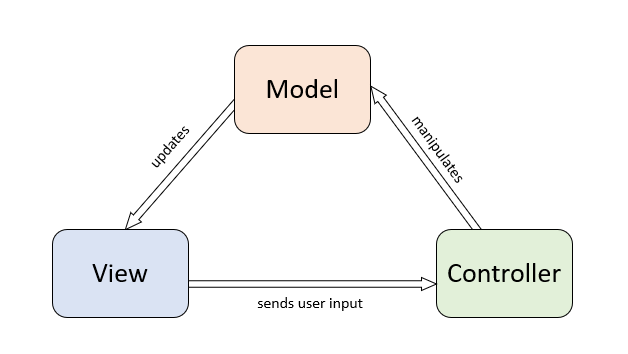
\includegraphics[width=15cm,height=7.5cm,keepaspectratio]{2GrundlagenX/Bilder/MVCArchitecture.png}
    \caption{MVC Architektur Diagramm \cite{mvcbild.2020}}
    \label{pic:mvcdiagram}
\end{figure} 
Im Falle dieser Abbildung wurde das Strukturmuster \ac{MVC} ausgewählt, welches die zu sehenden Komponenten in drei in sich 
geschlossene und unabhängige Fragmente unterteilt die miteinander interagieren. 
\\ 
\linebreak
Neben der Strukturierung von Systemen und Applikationen kann die Modellierung einer Softwarearchitektur auch dabei helfen eine Architektur genauer 
zu beschreiben und zu dokumentieren. Ebenso können Diagramme auch das Management sowie die Planung beeinflussen und verstärken. Die Modellierung 
der Softwarearchitektur stellt somit keinen Selbstzweck dar, sondern bietet einen Mehrwert indem es zur Verständigung, Dokumentation und 
Kommunikation zwischen Entwicklern und Kunden zusätzlich beiträgt. 
\\ 
Durch die Modellierung der Architektur kann frühzeitig eine sinnvolle Evaluierung und Bewertung des Entwurfs durchgeführt werden. Mit diesen 
entstehenden Bewertungen können folgende Schritte besser geplant und umgesetzt werden. 
\\ 
\linebreak
Eine weitere Variante, bzw. Ausprägung der Software-Architektur ist die Modulare Software Architektur (siehe Abschnitt \ref{chap:Modulare Software Architektur}).
Viele Softwarearchitekturen lehnen sich an das Prinzip der Modularen Architektur an und nehmen diese als Grundlage.
\subsection{Modulare Software Architektur}
\label{chap:Modulare Software Architektur}
Der Begriff der Modularität beschreibt den Hauptteil der Architektur. Modularität bezeichnet die Aufteilung eines großen Ganzen in 
mehrere kleinere Teile, die als Module, Komponenten oder Bausteine beschrieben werden. Verschiedene Teile können bei geeigneter Funktion 
und Kompatibilität zusammengeführt werden oder über entsprechend definierte Schnittstellen interagieren. 
\\ 
Unter der allgemeinen modularen Software-Architektur, bzw. Programmierung, versteht man ein Programmierparadigma. Dabei sollte die Software aus 
systematisch und logisch aufgeteilten Teilblöcke bestehen, diese werden Module oder Bausteine genannt. Der Aufbau der modularen Software kann 
praktisch in allen imperativen Programmiersprachen \footnote{Programmierparadigma, das aus einer Folge von Anweisungen besteht.} 
Anwendung finden. Durch Modularität soll die Software bessere Kontrollierbarkeit, Übersichtlichkeit und Testbarkeit innerhalb großer 
Softwareprojekte gewährleisten. So sind die einzelnen Bausteine an sich unabhängig und für sich selbst zuständig, trotz dessen können 
diese mit weiteren Bausteinen kombiniert und verschachtelt werden. 
\\ 
In der Entwicklung sind die einzelnen Module eigenständig und separat zu planen, programmieren und testen. Dadurch ist der Rahmen des 
einzelnen überschaubar und leicht zu praktizieren. Nach erfolgreicher Testung der Module können die Einzelteile als eine Anwendung 
zusammengeführt werden, indem die einzelnen Module logisch über Schnittstellen verknüpft werden. Erst nach diesem Schritt ist die 
entstehende Applikation vollständig einsatzbereit.
\\ 
Die modulare Programmierung gilt als Erweiterung des prozeduralen Ansatzes, dabei sind die Module in kleineren Ansätzen auf die Klassen 
der objektorientierten Programmierung zurückzuführen. \cite{modularesoftware.2018s}
\\
Um eine Software-Architektur übersichtlich und strukturiert umzusetzen, gibt es demzufolge Entwurfsmuster, engl. Patterns, die zusätzlich für 
Ordnung innerhalb der Architektur sorgen. Ein für die Ausarbeitung relevantes Muster ist das MVVM-Pattern. (siehe \ref{chap:MVVM})

\subsection{MVVM}
\label{chap:MVVM}
Das Model-View-ViewModel-Pattern ist, wie bereits erwähnt, ein Architekturmuster das den Entwicklern als Vorlage dient, um ordnungsgemäße, 
standardisierte und strukturierte grafische Oberflächen und das dahinterstehende logische System zu entwickeln. Es wird besonders für 
interaktive Systeme eingesetzt. Das MVVM-Muster wird allgemein als Weiterentwicklung des bekannten MVC-Patterns (der Abbildung \ref{pic:mvcdiagram} zu entnehmen) angesehen. 
\\
Grundlegend ist das Model-View-Controller-Muster, MVC, für die klare Abgrenzung zwischen Daten, deren Darstellung und Präsentation und den 
Nutzerinteraktionen für die graphischen Benutzeroberflächen gedacht. 
\\ 
\linebreak
Demnach ist auch das Model-View-ViewModel-Muster daran angelehnt, die Benutzeroberfläche von deren Logik zu trennen. Durch diese Trennung 
ist eine erhöhte Wartbarkeit und Testbarkeit gewährleistet. Die ermöglichte parallele Arbeitsweise von UI-Designern und Entwicklern 
unterstützt deren Arbeitsfluss und beschleunigt den Entwicklungsprozess. \cite{mvvmentwickler.2010s} 
\\ 
\linebreak
Die Logik der Anwendung wird in den ViewModel-Klassen (\ref{sec:ViewModel}) dargestellt und dienen als Kommunikationsschnittstelle zwischen 
dem Model, dem Datenhalter, und der View, der Datenrepräsentation. Durch die Unabhängigkeit der einzelnen Module kann ein Unit Test vereinfacht 
durchgeführt werden, mitunter ein großer Vorteil des Patterns. 
\\ 
Die Ebenen, die das MVVM-Pattern enthält, werden in Abbildung (\ref{pic:mvvmdiagram}) grafisch aufgeführt.
\begin{figure}[hbt!]
    \centering
    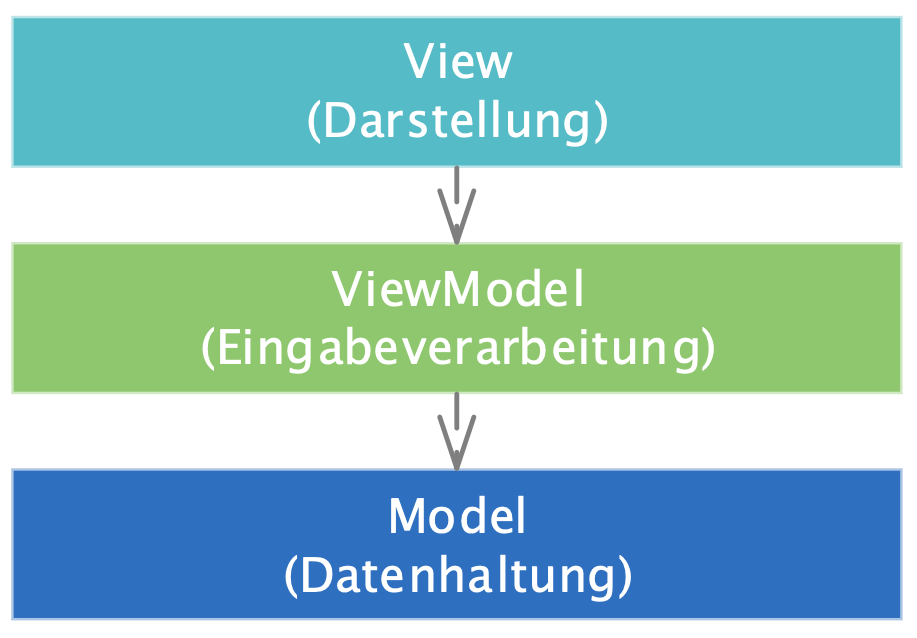
\includegraphics[width=15cm,height=7.5cm,keepaspectratio]{2GrundlagenX/Bilder/mvvmDiagramm.png}
    \caption{MVVM Architektur Diagramm \cite{mvvmDiagramm.2015n}}
    \label{pic:mvvmdiagram}
\end{figure} 
Die View-Ebene stellt die Informationen der Benutzeroberfläche dar, fängt die Benutzereingaben ab 
und gibt diese über Datenbindungen dann an das darunterliegende ViewModel weiter. Die View-Klasse enthält lediglich die Komponenten die 
die Oberfläche optisch aus machen und die dazugehörigen Datenbindungsschnittstellen, um die Informationen übergeben zu können.
Ebenso werden über diese Schnittstelle Informationen geladen, um diese auf der Oberfläche repräsentieren zu können. 
Diese Vorgehensweise erleichtert das Austauschen der View ohne den Code generell zu ändern. 
\\ 
\linebreak 
Die ViewModel, bereits in Kapitel (\ref{sec:ViewModel}) beschrieben, ist dafür zuständig die Daten zwischen der persistierten Speicherung 
und der Repräsentation zu transferieren. Es stellt das Model für die View dar und gibt das eigentliche Model nach außen.
\\ 
\linebreak 
Die unterste Ebene, das Model, bzw. die Datenhaltung, stellt die Abbildung der Daten dar und giltet nicht  als reine Abbildung der Datenquelle. 
Diese Daten werden für die visuelle Anwendung auf der View-Ebene benötigt und durch die ViewModel-Ebene bereitgestellt. Darüberhinaus können die 
Daten von dem Nutzer über die View manipuliert und an das Model zurückgegeben werden. Durch diese Möglichkeiten ist vorausgesetzte, dass das Model 
folgende Funktionalitäten bereitstellen sollte \cite{mvvmAufbau.2016}:
\begin{itemize}
    \item Validierung der Daten
    \item  Benachrichtigung bei Eigenschafts-Änderungen
    \item Verarbeitung von Business-Rules
\end{itemize} 
Sozusagen dient das Model als Schnittstelle zwischen der anhängenden Datenbank und dem ViewModel, welches die Daten hält. 
Dazu kommt, dass das Model festlegt wie die Objekte aufgebaut sind, d.h. dort wird festgelegt welchen Informationen das Objekt beinhaltet. 
\\ 
\linebreak
Basierend auf der Grundlage des Model-View-ViewModel-Patterns wurde die für das Projekt anvisierte Architektur, Android Architecture Components (\ref{chap:AAC}), 
entwickelt.  
\subsection{Android Architecture Components}
\label{chap:AAC}



\section{Datenmodellierung}
\label{chap:Datenmodellierung}